\chapter{Human Visual System}%
\label{ch:hvs}

It is essential to understand how the human visual system (HVS) functions to produce colour images of a scene on a digital camera that resembles how a human might perceive it. Figure \ref{fig:humaneye} shows a cross-section of the human eye. Note that many parts of the human eye have direct correspondences in a typical digital camera, such as the lens and the cornea, which focus an inverted image onto the retina, similar to how a lens in a digital camera focuses the image on a sensor. The ciliary muscles attached to the lens can also change their shape when focusing at different distances is required, much like how camera lenses with variable focal lengths work. The pupil and iris together create a system comparable to a digital camera's adjustable aperture, controlling the amount of light entering the eye.

\begin{figure}
    \centering
    \pdftooltip{
\includegraphics[width=0.7\textwidth]{figures/eye.eps}}{eye cross-section}
    \caption{Cross-section of the human eye \cite{humaneye}.}
    \label{fig:humaneye}
\end{figure}

\section{Retinal receptors}

As is explained in \cite[4-5]{measuringcolour}, our visual system adapts to different lighting conditions using rods and cones. The rods, active in low-light situations such as under moonlight, provide monochromatic "night vision", known as scotopic vision. In contrast, the cones function in well-lit conditions, like daylight, enabling us to perceive colours. This colour perception is part of the photopic vision system. The distinction in colour perception between scotopic and photopic vision is that there are three types of cones, each sensitive to a different wavelength range, as opposed to only one kind of rod.

On the boundaries of these two conditions, known as the mesopic vision, both the rods and cones are active, resulting in a phenomenon where colours are visible but appear darker and blueish. This is known as the Purkinje effect and is shown in Figure \ref{fig:purkinje} \cite[5]{measuringcolour}.


\begin{figure}
    \centering
    \pdftooltip{\includegraphics[width=\textwidth]{figures/Purkinje_effect_side_by_side.png}}{Purkinje}
    \caption{Purkinje Effect from left to right: Photopic Vision, Mesopic Vision and Scotopic Vision \cite{purkinje_effect}.}
    \label{fig:purkinje}
\end{figure}

\section{Spectral sensitivity}
\label{sec:responsivity}

To model the human eye computationally, it is essential to quantify how sensitive the eye is at some wavelength relative to some other wavelength. A standard was published in 1931 consisting of data collected by Wright and Guild from psychovisual experiments on subjects with standard vision under photopic vision \cite{wrightetguild}. The subjects were asked to match a reference light at some known wavelength, using a combination of three different lights with wavelengths of 435.8, 546.1 and 700 nm, corresponding roughly to the blue, green and red wavelengths, respectively. 

These results from the two groups of observers were combined and standardized by CIE in 1931. The so-called CIE 1931 RGB colour matching functions are shown in Figure \ref{fig:ciergb}, which denote the amount of each colour to match the reference light \cite{observer}, \cite{fairman1997cie}. The colours red, green and blue are also known as the primaries of this colour space. The choice of three primaries posed some problems, as it's impossible to reproduce every colour with an additive mixture of fixed three colours. As a result, for example, red is negative in the 450-550 nm range, as some of it had to be added to the reference light instead of adding to the other two primaries \cite[65]{colorimetry}.

To solve the aforementioned issues and simplify computations, at the same time in 1931, CIE introduced another set of colour-matching functions based on the previous, but with the requirement that all the functions should be strictly positive, and one of them should correspond to the luminance of the colour \cite[32-33]{measuringcolour}. Thus, another, much more widely used, set of functions, the CIE 1931 XYZ colour matching functions, was published. The functions are shown in Figure \ref{fig:xyz}.

\begin{figure}
    \centering
    \pdftooltip{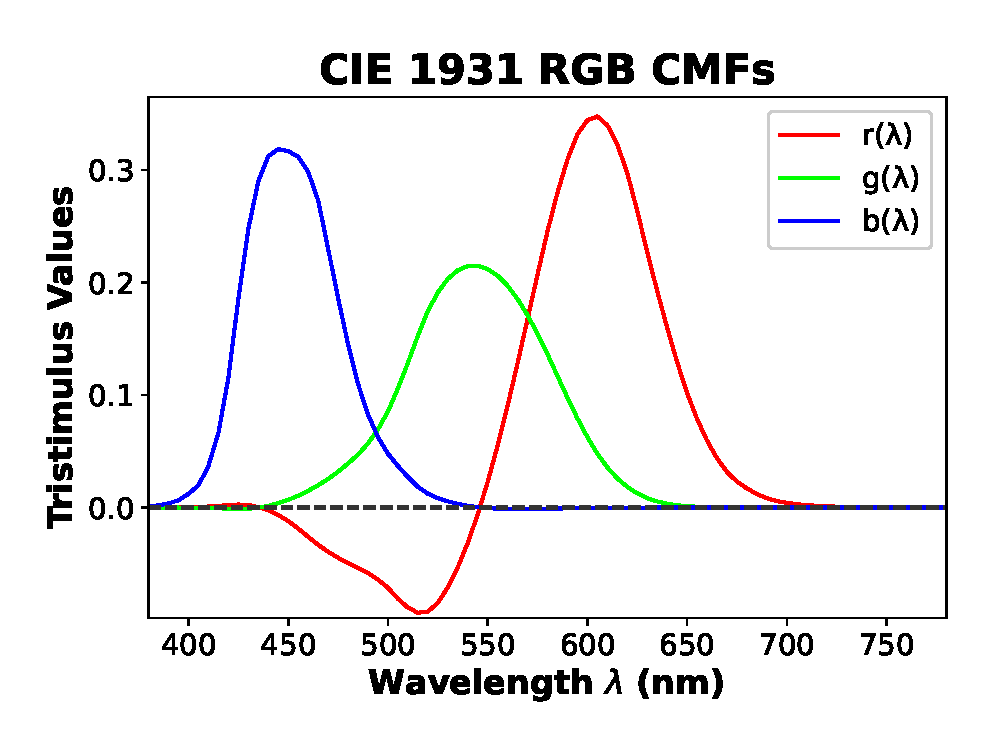
\includegraphics[width=\textwidth]{figures/cie_rgb.eps}}{CIE RGB CMFs}
    \caption{CIE RGB colour-matching functions \cite{cie1931}.}
    \label{fig:ciergb}
\end{figure}

\begin{figure}
    \centering
    \pdftooltip{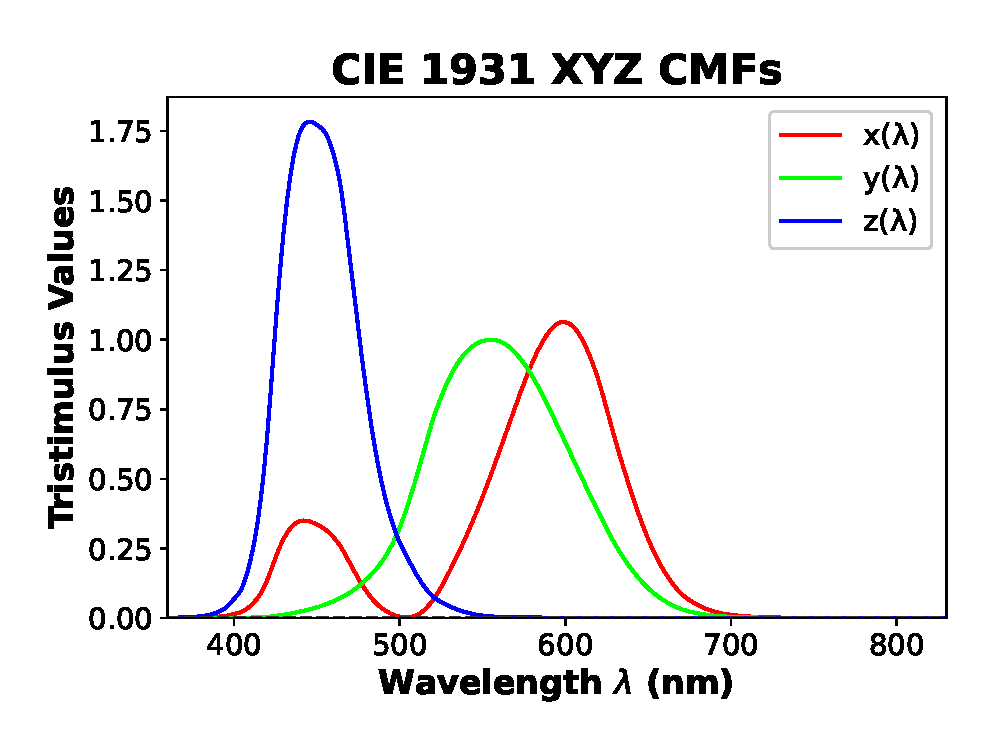
\includegraphics[width=\textwidth]{figures/cie_xyz.eps}}{CIE XYZ CMFs}
    \caption{CIE XYZ colour-matching functions \cite{cie1931}.}
    \label{fig:xyz}
\end{figure}

As a note, spectral sensitivity and responsivity are often used interchangeably in the literature. However, responsivity is more clearly defined as the current generated by optical power, whereas the definition of sensitivity is ambiguous. Here, we talk about sensitivity when the output is relative and thus unitless, whereas we use responsivity when the output is quantifiable and expressed in specific units. \cite{Paschotta2005responsivity}, \cite{Paschotta2019sensitivity}

\section{Tristimulus values}
\label{sec:tristimulus}

What colour we perceive an object to be is determined by the type of material the light is incident on before reaching our eye. Both have different spectral properties that describe their interaction, and light can, for example, reflect from and transmit or absorb into the object, or all of them can happen simultaneously. 

The light that reaches our eye, known as the stimulus spectrum, can be determined by multiplying the object's reflectance spectrum and the light source's spectral power distribution (SPD). The human eye then performs a weighted sum of the incident stimulus and the colour matching functions from Figure \ref{fig:xyz}, resulting in the XYZ tristimulus values. This process is further visualized in Figure \ref{fig:light}.


Mathematically, the tristimulus value $T$ corresponding to either $X$, $Y$ or $Z$ is then given by

\begin{subequations}
\begin{align}
\label{eq:tristimulus}
X = k \int_{380}^{780} E(\lambda) R(\lambda) S_X(\lambda) \, d\lambda \\
Y = k \int_{380}^{780} E(\lambda) R(\lambda) S_Y(\lambda) \, d\lambda \\
Z = k \int_{380}^{780} E(\lambda) R(\lambda) S_Z(\lambda) \, d\lambda,
\end{align}
\end{subequations}

Where $E(\lambda)$ is the spectral power distribution (SPD) of the illuminant, $R(\lambda)$ is the spectral reflectance of the object, and $S_T(\lambda)$ is the sensitivity of the cones for tristimulus value \( T \) (either \( X, Y, \) or \( Z \)). 

\begin{figure}
    \centering
    \pdftooltip{\includegraphics[width=\textwidth]{figures/stimulus.png}}{Color Formation}
    \caption{Colour formation model}
    \label{fig:light}
\end{figure}

As one of the components, $Y$, corresponds to the luminance of the colour, it makes sense to normalize it between 0 and 100 to treat it as a percentage. The normalization factor $k$ can be computed as the response of the Y channel to light reflected from a perfectly white surface with Lambertian reflectance as follows.

\begin{equation}
\label{eq:normalization}
 k = \frac{100}{\int_{380}^{780} E(\lambda) S_Y(\lambda) \, d\lambda},
\end{equation}

Where $100$ is a scaling factor, $E(\lambda)$ is the spectral power distribution of a given illuminant, and $S_Y(\lambda)$ is the cone sensitivity for Y \cite{rowlands2020physics}. Note that $1$ is often used for simplicity as the scaling factor in numerical computation.

\subsection{Metamerism}
\label{ss:metamerism}
Even though the CIE XYZ colour matching functions provide an elegant and standardized way to quantify the response of an average human, the fact that the functions are a little different for each human poses some exciting problems \cite[118]{measuringcolour}. 

Figure \ref{fig:metamerism} demonstrates this phenomenon for other patches under various light sources, with the right side of the patch showing the colour under sunlight and the left side showing it under the corresponding light source written in the leftmost column. It is clear that the patches all look similar under sunlight, but we notice significant changes when observing them under different light sources. This phenomenon is known as metamerism. Depending on the illumination conditions, two objects with separate spectral properties can look the same, completely different, or similar \cite[117-121]{metamerism}.

\begin{figure}
    \centering
    \pdftooltip{\includegraphics[width=\textwidth]{figures/metamerism.png}}{Metamerism}
    \caption{Simulation of Metameric Surfaces under different Illuminants \cite{metamerism}.}
    \label{fig:metamerism}
\end{figure}

\section{Chromatic Adaptation}
\label{sec:chromaticadaptation}
Although one would assume that the tristimulus system is enough to model the HVS, the human eye can adapt its sensitivities under different illuminant conditions. Even though the same scene under two different illuminants will produce distinct tristimulus values, the human visual system will often perceive them as having been the same colours. For example, a white sheet of paper will look white under sunlight and a fluorescent light source. This feature is called chromatic adaptation \cite[146-149]{fairchild}.

Much research has addressed this phenomenon during the past century, and the current ideas only approximate the complex biological process. Johannes von Kries proposed the most common and oldest hypothesis in 1902, where he suggested that the human visual system adapts to changing illumination by applying gain multipliers to the cone sensitivities \cite[168-171]{fairchild}. This effectively results in a set of coefficients for each illuminant and can be mathematically formulated as follows

\begin{equation}
\label{eq:vonkries}
\begin{bmatrix}
L' \\
M' \\
S' \\
\end{bmatrix}
=
\begin{bmatrix}
1/k_L & 0 & 0 \\
0 & 1/k_M & 0 \\
0 & 0 & 1/k_S \\
\end{bmatrix}
\begin{bmatrix}
L \\
M \\
S \\
\end{bmatrix}
,
\end{equation}

Where $L$, $M$, $S$ are the responses of the Long, Medium and Short wavelength cones to the original light source, $L'$, $M'$, $S'$ are the transformed responses after adaptation, and $k_L$, $k_M$, $k_S$ are the von Kries coefficients. The can be computed by substituting the Y channel sensitivity with cone sensitivities in formula \ref{eq:normalization}, using an appropriate scaling factor instead of $100$. This formula effectively removes the effect of the illuminant and ensures that neutral objects have the same response under every light source.

Even in his publication, von Kries argued that his proposal was a gross oversimplification. However, in practice, the method is still applied and has been proven to be an excellent approximate \cite[170-171]{fairchild}. For example, consumer digital cameras often follow this model when simulating chromatic adaptation. More sophisticated models of chromatic adaptation exist, such as the Retinex Theory \cite{land1977retinex} or Bradford Transform \cite{lam1985metamerism}. Still, as we do not emphasize chromatic adaptation in this thesis, we only consider the von Kries transform in subsequent chapters for practical purposes.


\section{Colour Spaces}

Colour spaces are a fundamental element in colour science. They establish the primary colours and the geometric representation of the range of colours that can be reproduced within a specific colour space. Additionally, they often include criteria for quantifying the differences between sets of colours. For instance, the colour matching functions depicted in Figure \ref{fig:xyz} constitute the CIE XYZ 1931 colour space, as defined by \cite{cie1931}.

Colour spaces can roughly be divided into device-independent and device-dependent colour spaces. In the former, colour values are not tied to any particular device. They are instead based on human visual perception or standardized models, while in the latter, the interpretation of specific colour values can vary wildly across devices.

\subsection{Device-independent colour spaces}

\textbf{Device-independent colour spaces} can be divided into three subcategories: reference, output-referred, and perceptually uniform colour spaces \cite[ch.~4.1-4.5]{rowlands2020physics}. The last two are always related to the first by some known transformation. 

Since colour values in device-independent colour spaces have universal meaning, they can also be easily visualized, and the set of reproducible colours can be compared. However, as colour spaces are three-dimensional and form complex shapes, one dimension is often dropped for visualization purposes, resulting in a \textbf{chromaticity diagram} \cite[42-44]{measuringcolour}.

Three different colour spaces are shown on a chromaticity diagram in \ref{fig:gamut}. The filled horseshoe-shaped figure corresponds to the colours a human could theoretically see. At the same time, the two smaller triangles, in this case, Adobe Adobe RGB \cite{adobeRGB} and sRGB \cite{sRGB}, are subspaces of the former. The colours inside the outlined shapes form the gamut of a colour space, which contains the set of colours reproducible by the space or a system.

\begin{figure}
    \centering
    \pdftooltip{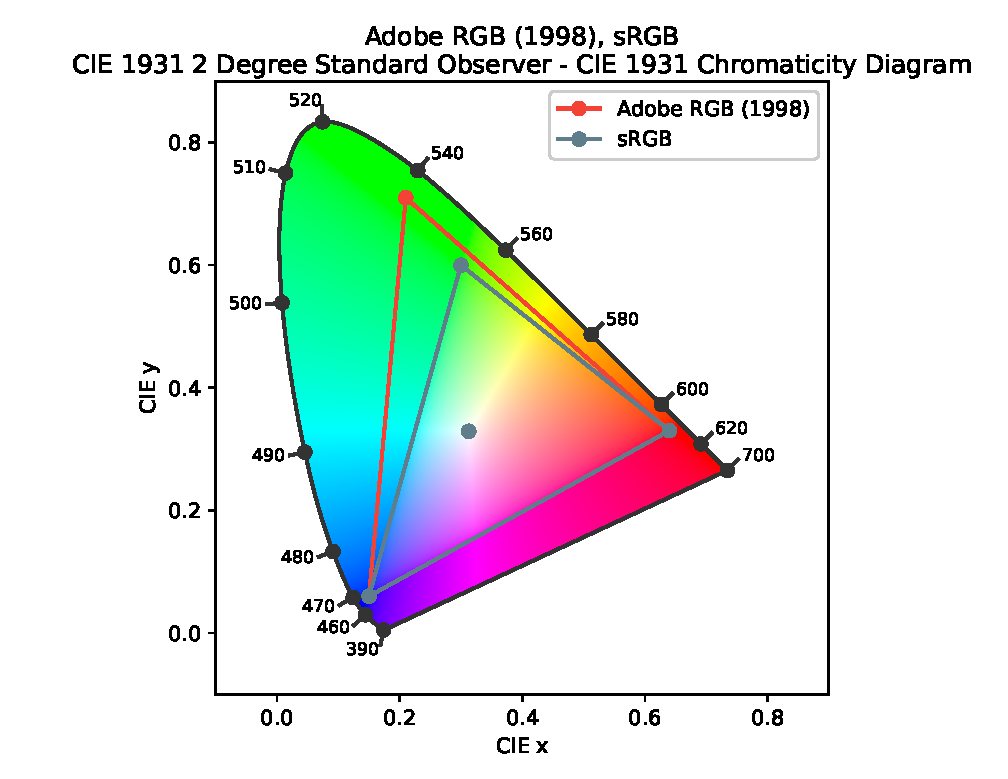
\includegraphics[width=\textwidth]{figures/gamut.eps}}{ Gamut}
    \caption{CIE XYZ \cite{cie1931}, Adobe RGB \cite{adobeRGB} and sRGB \cite{sRGB} colour gamuts on a chromaticity diagram}
    \label{fig:gamut}
\end{figure}

\textbf{Reference colour spaces} are defined to contain all visible colours producible by the human eye. These include 
for example the CIE XYZ colour space seen in Figure \ref{fig:gamut}. Reference spaces allow us to move to other linearly related spaces by changing their basis, which makes them convenient. Furthermore, they are often used as target colour space when the input is in camera-specific colour space. For example, the following transformation takes us from the CIE XYZ reference colour space to an output-referred sRGB colour space \cite{brucelindbloom}:

\begin{equation}
\text{XYZ} \rightarrow \text{sRGB} = 
\begin{bmatrix}
3.2404542 & -1.5371385 & -0.4985314 \\
-0.9692660 & 1.8760108 & 0.0415560 \\
0.0556434 & -0.2040259 & 1.0572252
\end{bmatrix}
\end{equation}


\textbf{Output-referred colour space} defines a standard for output devices, ensuring manufacturers interpret a set of colour values similarly. Otherwise, two manufacturers could use proprietary formats; thus, an image would produce different colours on different display devices. To this date, output-referred colour spaces occupy only a subset of the reference colour spaces, partially because an additive mixture of three primaries cannot represent all colours visible to humans, as was discussed in \ref{sec:responsivity}. This is the case for the most common colour spaces, such as sRGB and Adobe RGB, based on red, blue and green primaries. Figure \ref{fig:gamut}.

It is often necessary to measure the difference between two colours, such as to compare how accurately an algorithm produces colours compared to how an observer would have seen them. However, even when using reference colour spaces with a geometrical interpretation, it is not guaranteed that two pairs of colours with the same distance will appear equally different to an observer \cite[48-49]{measuringcolour}. To optimize algorithms for perceptual quality, it is essential to create colour spaces that consider this.

\textbf{Uniform colour spaces}, as described in \cite[53-57]{measuringcolour}, attempt to ensure that a set of colour pairs with the same perceptual distance have the same distance in terms of geometrical distance. Two colour spaces, introduced in 1976, are primarily used to this date: CIELUV and CIELAB \cite{cielab}. In both spaces, $L$ refers to the lightness of the colour (luminance in greyscale), while $u,v$ and $a,b$ are the chromaticity coordinates. Hue-angle (dominant wavelength) and chroma (purity of the colour) can be computed from the chromaticity coordinates. For CIELUV, saturation can also be computed \cite[51]{measuringcolour}, although chroma is often used instead.

Perhaps most importantly, uniform colour spaces can approximate perceptual differences between colours. Often, these metrics define a unit for \textbf{just noticeable difference (JND)}, which, in colour science, refers to the amount of colour that would have to be changed before an average observer notices a difference. Since \textbf{CIELUV} and \textbf{CIELAB} are approximately uniform, the easiest metric to implement is the Euclidean distance between two colours. In the CIELAB space, this is known as the CIE76 or $\Delta E^{*}$ formula and is given by

\begin{equation}
\label{eq:cie76}
\Delta E^* = \sqrt{(L_2^* - L_1^*)^2 + (a_2^* - a_1^*)^2 + (b_2^* - b_1^*)^2}
,
\end{equation}

where $\Delta E^*$ is the total colour difference, $L_1^*$ and $L_2^*$ are the lightness values of the first and second colours, 
$a_1^*$ and $a_2^*$ are the $a^*$ chromaticity values of the first and second colours
$b_1^*$  and $b_2^*$ are the $a^*$ chromaticity values s of the first and second colours.

Since then, even more accurate formulas have been introduced, such as the CIEDE2000 colour difference formula \cite{ciede2000dev}.

\section{Device-dependent colour spaces}

 Each device produces its own set of RGB values, even if they were used to capture precisely the same scene under constant conditions. It is then up to the camera manufacturer to ensure that the values stored in an image conform to some standard.
 
Similar to there being variety in the responses of the human eye across the population to some stimuli, there is also variation in the colour responses produced by a digital camera, even if they are produced precisely the same \cite{walowit2019best}. These differences are often mitigated by performing calibration per camera unit, adjusting, for example, the colour correction matrix multipliers discussed as will be discussed in \ref{ss:cc}.